\chapter{Installazione}
\label{Installazione}
\thispagestyle{empty}

%\section{Introduzione}
L'installazione di ShareLaTeX avviene su una macchina virtuale all'interno di un server del laboratorio AImageLab. Tale macchina ha nome \verb|sharelatex| ed esegue il sistema operativo Ubuntu 18.04 LTS, il più recente alla data corrente. Il sistema è accessibile sia dall'interno dell'ateneo (se collegati alla rete locale), sia dall'esterno, grazie all'apertura della porta 443, all'indirizzo \url{sharelatex.ing.unimore.it}. L'installazione e la configurazione sono avvenute seguendo i passi sotto riportati. L'attuale amministratore del sistema è il Dott. Federico Bolelli.

\section{Docker}
Per il progetto ShareLaTeX si è optato per l'installazione di Docker CE, in quanto non risultano necessarie le funzionalità aggiuntive dell'Enterprise Edition, rivolte invece alle grandi imprese. L'installazione può avvenire in diversi modi, come indicato nella guida ufficiale disponibile al sito \url{docs.docker.com/install/linux/docker-ce/ubuntu/}. Si è scelto di utilizzare il metodo raccomandato da Docker, ovvero tramite i loro repository.

\subsection{Download}
Aggiornare l'indice dei pacchetti di \verb|apt-get|.
\begin{lstlisting}
sudo apt-get update
\end{lstlisting}
Installare i pacchetti necessari per permettere a \verb|apt-get| di utilizzare un repository su HTTPS.
\begin{lstlisting}
sudo apt-get install \ 
    apt-transport-https \
    ca-certificates \
    curl \
    software-properties-common
\end{lstlisting}
Aggiungere la chiave GPG ufficiale di Docker.
\begin{lstlisting}
curl -fsSL https://download.docker.com/linux/ubuntu/gpg | sudo apt-key add -
\end{lstlisting}
Verificare di possedere la chiave con il fingerprint\\
\verb|9DC8 5822 9FC7 DD38 854A E2D8 8D81 803C 0EBF CD88|\\
cercando gli ultimi 8 caratteri della fingerprint.
\begin{lstlisting}
sudo apt-key fingerprint 0EBFCD88
\end{lstlisting}
L'output dovrebbe essere:
\begin{lstlisting}
pub   4096R/0EBFCD88 2017-02-22
Key fingerprint = 9DC8 5822 9FC7 DD38 854A E2D8 8D81 803C 0EBF CD88
uid     Docker Release (CE deb) <docker@docker.com>
sub     4096R/F273FCD8 2017-02-22
\end{lstlisting}
Monstare il repository stabile. Il server ha un processore con architettura x64, pertanto sarà necessario imppostare \verb|arch=amd64| come segue.
\begin{lstlisting}
sudo add-apt-repository \
"deb [arch=amd64] https://download.docker.com/linux/ubuntu \
$(lsb_release -cs) \
stable"
\end{lstlisting}

\subsection{Installazione}
Installare l'ultima versione di Docker CE.
\begin{lstlisting}
sudo apt-get install -y docker-ce
\end{lstlisting}
Verificare che Docker CE sia installato correttamente avviando l'immagine \verb|hello-world|.
\begin{lstlisting}
sudo docker run hello-world
\end{lstlisting}


\section{Docker Compose}
Docker Compose non è incluso all'interno del pacchetto Docker precedentemente installato. La sua installazione è necessaria ai fini del progetto per poter gestire al meglio i tre container che strutturano l'applicazione: ShareLaTeX, MongoDB e Redis.
\begin{figure}[h]
    \centering
    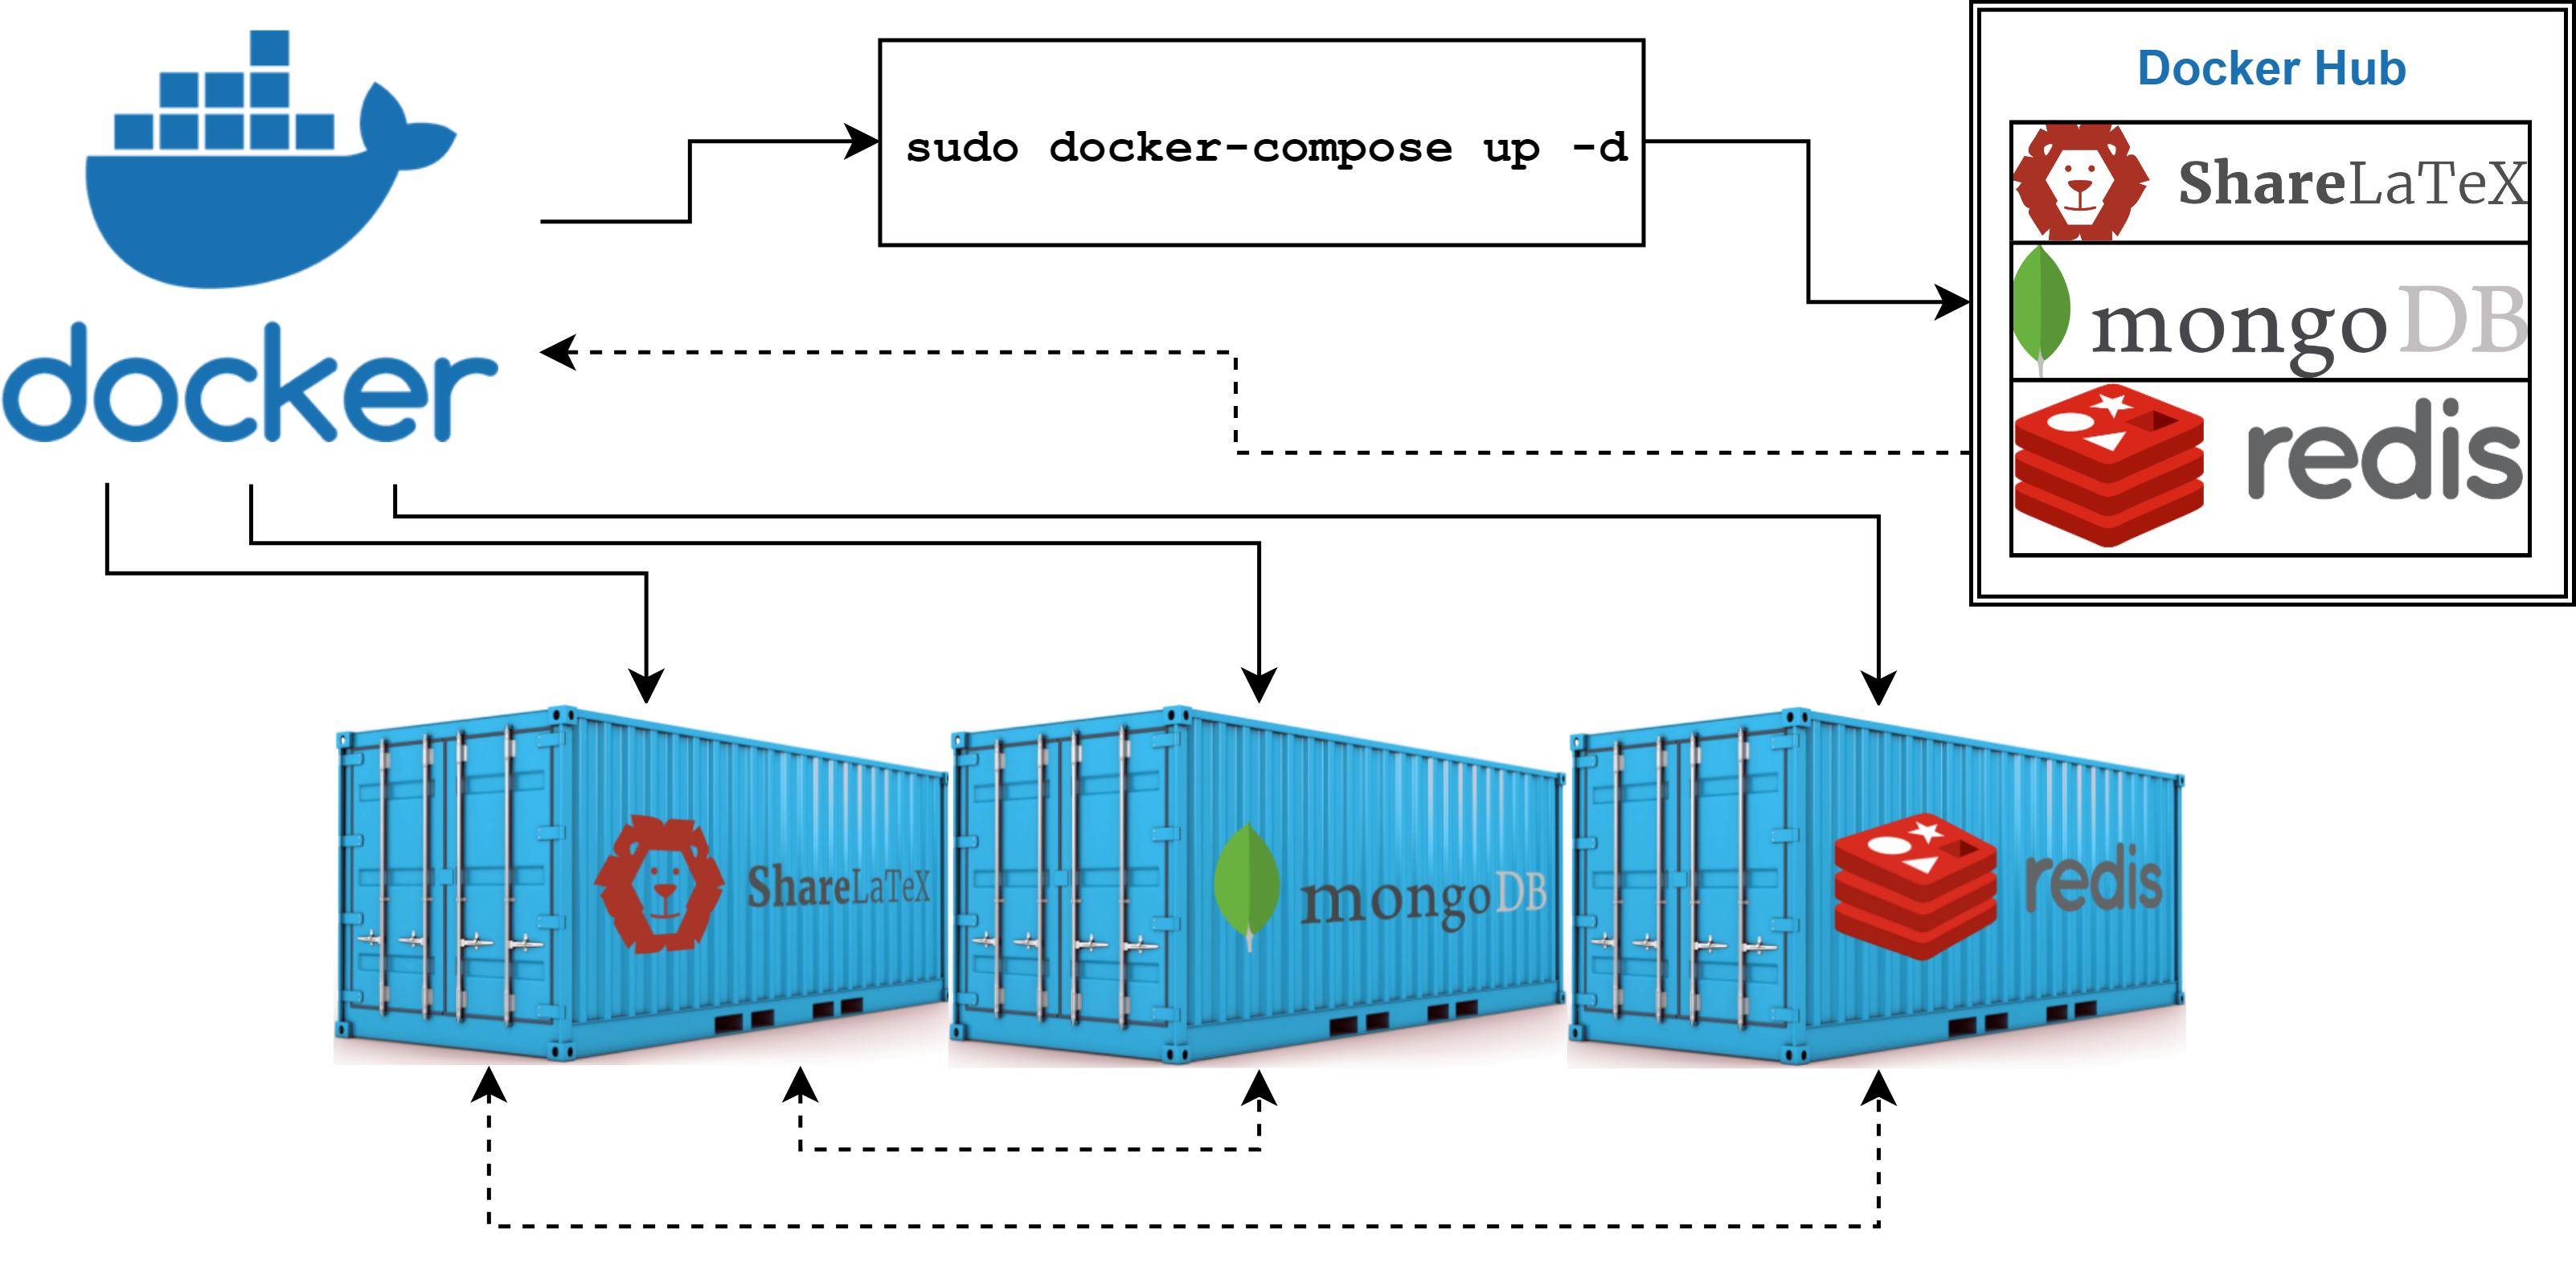
\includegraphics[scale=0.1]{immagini/docker_container_dependencies.png}
    \caption{Esecuzione di Docker Compose e dipendenze fra container}
    \label{fig:docker_compose_dipendenze}
\end{figure}

\subsection{Download e installazione}
Download di Docker Compose. Col seguente comando verrà installata la versione 1.21.2. Per installare un'altra versione del software, eventualmente più aggiornata, è necessario modificare l'indirizzo inserendo la versione richiesta. Per informazioni sull'ultima versione disponibile, visitare \verb|github.com/docker/compose/releases|.
\begin{lstlisting}
sudo curl -L https://github.com/docker/compose/releases/download/1.21.2/docker-compose-$(uname -s)-$(uname -m) -o /usr/local/bin/docker-compose
\end{lstlisting}
Applicare i permessi di esecuzione al file binario.
\begin{lstlisting}
sudo chmod +x /usr/local/bin/docker-compose
\end{lstlisting}
Testare la corretta installazione.
\begin{lstlisting}
docker-compose --version
\end{lstlisting}

\subsection{Configurazione}
Creare una directory dal nome \verb|sharelatex| e inserirvi \verb|docker-compose.yml|. Il template fornito dagli sviluppatori di ShareLaTeX per l'installazione tramite Docker è il seguente:
\lstinputlisting[caption={Template di docker-compose.yml}, captionpos=b, label=code:docker-compose.yml]{script/docker-compose-ridotto.yml}
Oltre a creare il container di ShareLaTeX, il file configura Redis e MongoDB. Inoltre fornisce una buona interfaccia per fornire impostazioni a ShareLaTeX\footnote{Si veda il capitolo \href{Configurazione}{Configurazione}.}.
\begin{lstlisting}
mkdir sharelatex
cd sharelatex
wget https://raw.githubusercontent.com/aimagelab/sharelatex/master/docker-compose.yml
\end{lstlisting}
Infine avviare i container di MongoDB, Redis e ShareLaTeX usando le impostazioni in \verb|docker-compose.yml|. L'opzione \verb|-d| serve per avviare i container in modalità "detached", ovvero in background.
\begin{lstlisting}
sudo docker-compose up -d
\end{lstlisting}
Per visualizzare i container attualmente attivi, eseguire seguente comando.
\begin{lstlisting}
sudo docker ps
\end{lstlisting}